% schem_overview: overview schematic (full width, 7.00 x 2.80 in, included at 100%).
% Left: one measurement model and the design rule. Right: three lanes,
% (a) correct a correlation, (b) compare models, (c) embedding reliability,
% read as baseline / check and response / outcome.
% Coordinates are inches from the bottom-left corner of the canvas.
% Build: pdflatex -interaction=nonstopmode -halt-on-error schem_overview.tex
%
% The caption is in the paper source, in the figure with \label{fig:overview}.
\documentclass[border=0.5pt]{standalone}
\usepackage{newtxtext,newtxmath}
\usepackage{xcolor}
\usepackage{tikz}
\usetikzlibrary{arrows.meta,decorations.pathreplacing}

% Macros copied from the paper's LaTeX macro file (only those used here).
\newcommand{\rhat}{\hat{\rho}}
\newcommand{\robs}{r_{\mathrm{obs}}}
\newcommand{\rplug}{\hat r_{\mathrm{plug}}}
\newcommand{\thetastar}{\theta^{\star}}
\newcommand{\clip}{\mathrm{clip}}
\newcommand{\Certified}{\textsc{certified}}
\newcommand{\ProtDep}{\textsc{protocol-dependent}}
\newcommand{\Refused}{\textsc{refused}}
\newcommand{\Declined}{\textsc{declined}}

% Palette (Okabe-Ito, as in figscripts/style.py).
\definecolor{ALG}{HTML}{0072B2}
\definecolor{PLUG}{HTML}{D55E00}
\definecolor{POOL}{HTML}{CC79A7}
\definecolor{ZERO}{HTML}{56B4E9}
\definecolor{REF}{HTML}{999999}
\definecolor{TEXT}{HTML}{000000}
\definecolor{TEXT2}{HTML}{555555}
\definecolor{GUIDE}{HTML}{CCCCCC}
\definecolor{FAINT}{HTML}{E0E0E0}
\definecolor{FILL}{HTML}{F2F2F2}

\newcommand{\sev}{\fontsize{7}{8.4}\selectfont}
\newcommand{\eig}{\fontsize{8}{9.6}\selectfont}

% Markers (base size 3.5pt), each centered on the given point.
\newcommand{\mCert}[1]{\fill[ALG] #1 circle (1.75pt);}
\newcommand{\mProt}[1]{\fill[PLUG] #1 ++(-2pt,-1.732pt) -- ++(4pt,0) -- ++(-2pt,3.464pt) -- cycle;}
\newcommand{\mRef}[1]{\filldraw[fill=white,draw=REF,line width=0.8pt] #1 circle (1.75pt);}
\newcommand{\mZero}[1]{\filldraw[fill=white,draw=ZERO,line width=0.8pt] #1 ++(-1.75pt,-1.75pt) rectangle ++(3.5pt,3.5pt);}
\newcommand{\mTwo}[1]{\fill[ALG] #1 ++(-1.75pt,-1.75pt) rectangle ++(3.5pt,3.5pt);}
\newcommand{\mPool}[1]{\fill[POOL] #1 ++(-2pt,0) -- ++(2pt,2pt) -- ++(2pt,-2pt) -- ++(-2pt,-2pt) -- cycle;}

% Gap axis of lane (b): 0.0392857 in per point (-8 points at x 2.30 in c1, 3.95 in c2).
\newcommand{\gs}{0.0392857}

\begin{document}
\frenchspacing
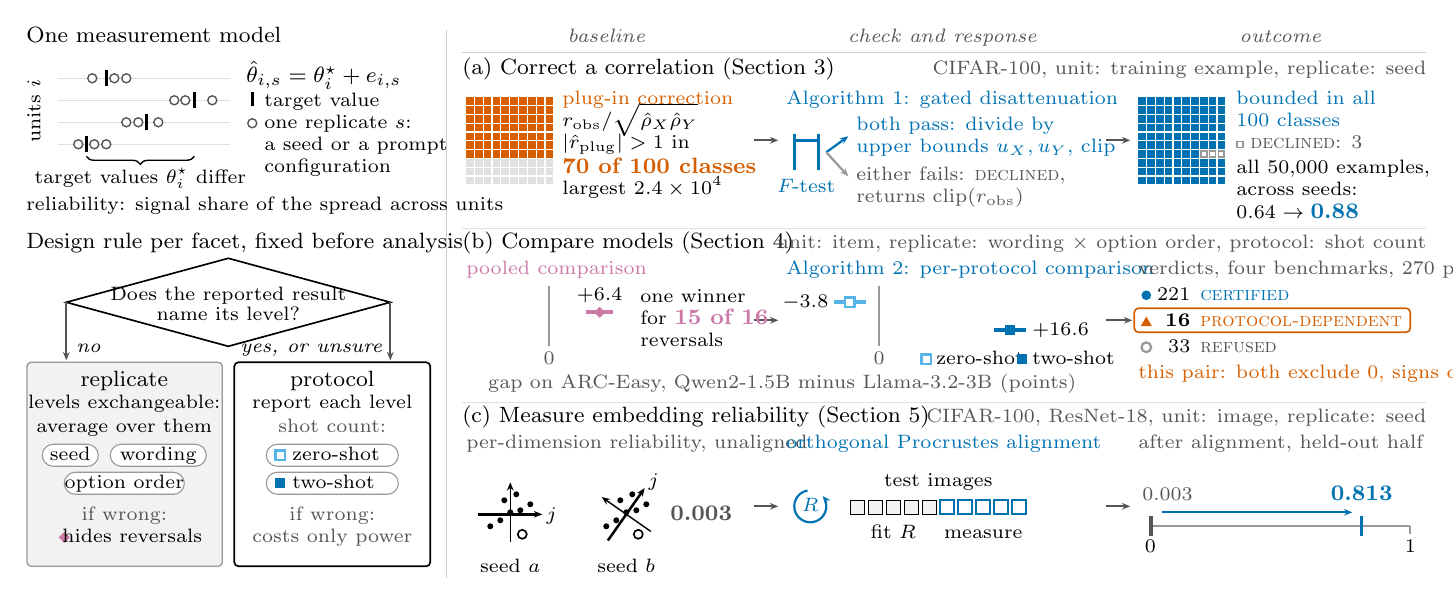
\begin{tikzpicture}[x=1in,y=1in,line width=0.6pt,line cap=butt,
  every node/.style={inner sep=0pt,outer sep=0pt,font=\sev,text=TEXT},
  L/.style={anchor=base west}, C/.style={anchor=base}, R/.style={anchor=base east},
  T/.style={font=\eig},
  flow/.style={draw=TEXT2,line width=0.6pt,-{Stealth[length=3pt,width=2.4pt]}},
  marr/.style={line width=0.8pt,-{Stealth[length=3pt,width=2.4pt]}},
  axj/.style={draw=TEXT,line width=0.9pt,-{Stealth[length=3pt,width=2.4pt]}},
  axo/.style={draw=TEXT,line width=0.5pt,-{Stealth[length=3pt,width=2.4pt]}},
  pill/.style={draw=REF,line width=0.4pt,fill=white,rounded corners=0.055in},
  rep/.style={draw=TEXT2,line width=0.5pt,fill=white}]
% canvas 7.00 x 2.80 in including the 0.5pt standalone border on each side
\useasboundingbox (0.5pt,0.5pt) rectangle ([shift={(-0.5pt,-0.5pt)}]7.00,2.80);

% ====================================================== grid
\draw[GUIDE,line width=0.4pt] (2.10,0.04) -- (2.10,2.78);
\draw[GUIDE,line width=0.4pt] (2.18,2.67) -- (7.00,2.67);
\draw[FAINT,line width=0.4pt] (2.18,1.79) -- (7.00,1.79);
\draw[FAINT,line width=0.4pt] (2.18,0.92) -- (7.00,0.92);
\node[C,text=TEXT2,font=\sev\itshape] at (2.90,2.72) {baseline};
\node[C,text=TEXT2,font=\sev\itshape] at (4.58,2.72) {check and response};
\node[C,text=TEXT2,font=\sev\itshape] at (6.27,2.72) {outcome};
% flow arrows: lane (a) at 2.23, lane (b) at 1.33 (middle of the boxed row), lane (c) at 0.40
\foreach \y in {2.23,0.40} {
  \draw[flow] (3.64,\y) -- (3.76,\y);
  \draw[flow] (5.40,\y) -- (5.52,\y);
}
\draw[flow] (3.64,1.33) -- (3.76,1.33);
\draw[flow] (5.40,1.33) -- (5.53,1.33);

% ====================================================== left block: measurement model
\node[L,T] at (0.00,2.72) {One measurement model};
% replicate offsets chosen so that every circle clears its target tick and its neighbours
\foreach \ry/\rt/\oa/\ob/\oc in {2.54/0.40/-0.07/0.04/0.10, 2.43/0.84/-0.10/-0.045/0.09,
                                 2.32/0.60/-0.10/-0.04/0.06, 2.21/0.30/-0.04/0.04/0.10} {
  \draw[FAINT,line width=0.3pt] (0.16,\ry) -- (1.02,\ry);
  \foreach \ro in {\oa,\ob,\oc} \draw[rep] (\rt+\ro,\ry) circle (0.0225);
  \draw[TEXT,line width=1.0pt] (\rt,\ry-0.04) -- (\rt,\ry+0.04);
}
\node[C,rotate=90] at (0.07,2.375) {units $i$};
\draw[TEXT,line width=0.5pt,decorate,decoration={brace,amplitude=0.04in}]
  (0.84,2.15) -- (0.30,2.15);
\node[C] at (0.57,2.015) {target values $\thetastar_i$ differ};
\node[L,T] at (1.10,2.52) {$\hat\theta_{i,s}=\thetastar_i+e_{i,s}$};
\draw[TEXT,line width=1.0pt] (1.13,2.40) -- (1.13,2.47);
\node[L] at (1.19,2.40) {target value};
\draw[rep] (1.13,2.315) circle (0.0225);
\node[L] at (1.19,2.29) {one replicate $s$:};
\node[L] at (1.19,2.18) {a seed or a prompt};
\node[L] at (1.19,2.07) {configuration};
\node[L] at (0.00,1.88) {reliability: signal share of the spread across units};

% ====================================================== left block: design rule
% title shares its baseline with the lane (b) title
\node[L,T] at (0.00,1.69) {Design rule per facet, fixed before analysis};
\filldraw[fill=white,draw=TEXT,line width=0.6pt]
  (0.20,1.42) -- (1.01,1.64) -- (1.82,1.42) -- (1.01,1.20) -- cycle;
\node[C] at (1.01,1.43) {Does the reported result};
\node[C] at (1.01,1.33) {name its level?};
\draw[flow] (0.20,1.42) -- (0.20,1.13);
\node[L,font=\sev\itshape] at (0.25,1.17) {no};
\draw[flow] (1.82,1.42) -- (1.82,1.13);
\node[R,font=\sev\itshape] at (1.78,1.17) {yes, or unsure};
% replicate bin (neutral box); same internal rhythm as the protocol bin
\filldraw[fill=FILL,draw=REF,line width=0.5pt,rounded corners=1.5pt]
  (0.0035,0.10) rectangle (0.98,1.12);
\node[C,T] at (0.49,1.00) {replicate};
\node[C] at (0.49,0.89) {levels exchangeable:};
\node[C] at (0.49,0.77) {average over them};
\draw[pill] (0.08,0.60) rectangle (0.36,0.71);  \node[C] at (0.22,0.628) {seed};
\draw[pill] (0.42,0.60) rectangle (0.90,0.71);  \node[C] at (0.66,0.628) {wording};
\draw[pill] (0.19,0.46) rectangle (0.79,0.57);  \node[C] at (0.49,0.488) {option order};
\node[C,text=TEXT2] at (0.49,0.33) {if wrong:};
\mPool{(0.19,0.245)}
\node[C] at (0.53,0.22) {hides reversals};
% protocol bin (emphasis box)
\filldraw[fill=white,draw=TEXT,line width=0.6pt,rounded corners=1.5pt]
  (1.04,0.10) rectangle (2.02,1.12);
\node[C,T] at (1.53,1.00) {protocol};
\node[C] at (1.53,0.89) {report each level};
\node[C,text=TEXT2] at (1.53,0.77) {shot count:};
\draw[pill] (1.20,0.60) rectangle (1.86,0.71);
\mZero{(1.27,0.655)}  \node[L] at (1.33,0.628) {zero-shot};
\draw[pill] (1.20,0.46) rectangle (1.86,0.57);
\mTwo{(1.27,0.515)}   \node[L] at (1.33,0.488) {two-shot};
\node[C,text=TEXT2] at (1.53,0.33) {if wrong:};
\node[C,text=TEXT2] at (1.53,0.22) {costs only power};

% ====================================================== lane (a)
\node[L,T] at (2.18,2.56) {(a) Correct a correlation (Section 3)};
\node[R,text=TEXT2] at (7.00,2.56) {CIFAR-100, unit: training example, replicate: seed};
% c1: plug-in correction, 70 of 100 classes impossible (vermilion); the other 30 plain light cells
\foreach \k in {1,...,100} {
  \pgfmathtruncatemacro\rr{(\k-1)/10}
  \pgfmathtruncatemacro\cc{mod(\k-1,10)}
  \pgfmathsetmacro\xx{2.20+0.044*\cc}
  \pgfmathsetmacro\yy{2.444-0.044*\rr}
  \ifnum\k<71
    \fill[PLUG] (\xx,\yy) rectangle ++(0.038,-0.038);
  \else
    \fill[FAINT] (\xx,\yy) rectangle ++(0.038,-0.038);
  \fi
}
\node[L,text=PLUG] at (2.68,2.41) {plug-in correction};
\node[L] at (2.68,2.30) {$\robs/\sqrt{\rhat_X\rhat_Y}$};
\node[L] at (2.68,2.19) {$|\rplug|>1$ in};
\node[L,font=\eig\bfseries,text=PLUG] at (2.68,2.065) {70 of 100 classes};
\node[L] at (2.68,1.96) {largest $2.4\times10^4$};
% c2: Algorithm 1
\node[L,text=ALG] at (3.80,2.41) {Algorithm 1: gated disattenuation};
\draw[ALG,line width=0.9pt] (3.84,2.08) -- (3.84,2.26) (3.96,2.08) -- (3.96,2.26);
\draw[ALG,line width=1.2pt] (3.84,2.23) -- (3.96,2.23);
\node[C,text=ALG] at (3.90,1.97) {$F$\kern-0.8pt-test};
\draw[marr,ALG] (4.00,2.17) -- (4.11,2.25);
\draw[marr,REF] (4.00,2.17) -- (4.11,2.05);
\node[L,text=ALG] at (4.15,2.28) {both pass: divide by};
\node[L,text=ALG] at (4.15,2.17) {upper bounds $u_X,u_Y$, clip};
\node[L,text=TEXT2] at (4.15,2.03) {either fails: \Declined,};
\node[L,text=TEXT2] at (4.15,1.92) {returns $\clip(\robs)$};
% c3: bounded in all 100 classes, declined in 3 (open cells, placed among the
% positions that are vermilion in c1; cells count classes and are not matched)
\foreach \k in {1,...,100} {
  \pgfmathtruncatemacro\rr{(\k-1)/10}
  \pgfmathtruncatemacro\cc{mod(\k-1,10)}
  \pgfmathsetmacro\xx{5.56+0.044*\cc}
  \pgfmathsetmacro\yy{2.444-0.044*\rr}
  \pgfmathtruncatemacro\op{and(\k>67,\k<71)}
  \ifnum\op=1
    \draw[REF,line width=0.6pt,fill=white] (\xx+0.0042,\yy-0.0042) rectangle ++(0.0296,-0.0296);
  \else
    \fill[ALG] (\xx,\yy) rectangle ++(0.038,-0.038);
  \fi
}
\node[L,text=ALG] at (6.05,2.41) {bounded in all};
\node[L,text=ALG] at (6.05,2.30) {100 classes};
\draw[REF,line width=0.6pt,fill=white] (6.0542,2.1942) rectangle (6.0838,2.2238);
\node[L,text=TEXT2] at (6.12,2.19) {\Declined: 3};
\node[L] at (6.05,2.065) {all 50,000 examples,};
\node[L] at (6.05,1.955) {across seeds:};
\node[L] at (6.05,1.84) {$0.64\to{}${\eig\bfseries\color{ALG}0.88}};

% ====================================================== lane (b)
\node[L,T] at (2.18,1.69) {(b) Compare models (Section 4)};
\node[R,text=TEXT2] at (7.00,1.69)
  {unit: item, replicate: wording $\times$ option order, protocol: shot count};
% Interval positions only (never printed): results/algo2_reported, rows
% (arc, Qwen2-1.5B-Instruct, Llama-3.2-3B-Instruct), times 100.
% pooled_pairwise.csv: gap 6.4429 [4.7136, 8.1723]
% pairwise.csv protocol 0 (zero-shot): gap -3.7500 [-5.7921, -1.7079]
% pairwise.csv protocol 1 (two-shot): gap 16.6358 [14.6232, 18.6484]
% c1: pooled comparison
\node[L,text=POOL] at (2.20,1.56) {pooled comparison};
\draw[REF,line width=0.5pt] (2.614,1.20) -- (2.614,1.50);
\draw[POOL,line width=1.4pt] ({2.614+4.7136*\gs},1.37) -- ({2.614+8.1723*\gs},1.37);
\mPool{({2.614+6.4429*\gs},1.37)}
\node[C] at (2.867,1.43) {$+6.4$};
\node[C,text=TEXT2] at (2.614,1.11) {0};
\node[L] at (3.07,1.42) {one winner};
\node[L] at (3.07,1.31) {for {\eig\bfseries\color{POOL}15 of 16}};
\node[L] at (3.07,1.20) {reversals};
% c2: Algorithm 2
\node[L,text=ALG] at (3.80,1.56) {Algorithm 2: per-protocol comparison};
\draw[REF,line width=0.5pt] (4.264,1.20) -- (4.264,1.50);
\draw[ZERO,line width=1.4pt] ({4.264-5.7921*\gs},1.42) -- ({4.264-1.7079*\gs},1.42);
\mZero{({4.264-3.7500*\gs},1.42)}
\node[R] at (4.01,1.395) {$-3.8$};
\draw[ALG,line width=1.4pt] ({4.264+14.6232*\gs},1.28) -- ({4.264+18.6484*\gs},1.28);
\mTwo{({4.264+16.6358*\gs},1.28)}
\node[L] at (5.03,1.255) {$+16.6$};
\node[C,text=TEXT2] at (4.264,1.11) {0};
\mZero{(4.50,1.135)}  \node[L] at (4.55,1.11) {zero-shot};
\mTwo{(4.98,1.135)}   \node[L] at (5.03,1.11) {two-shot};
\node[C,text=TEXT2] at (3.78,0.99) {gap on ARC-Easy, Qwen2-1.5B minus Llama-3.2-3B (points)};
% c3: verdicts over 270 pairs on four benchmarks
\node[L,text=TEXT2] at (5.56,1.56) {verdicts, four benchmarks, 270 pairs};
\draw[PLUG,line width=0.6pt,rounded corners=1.5pt] (5.54,1.27) rectangle (6.92,1.39);
\mCert{(5.60,1.455)} \node[R] at (5.82,1.43) {221};          \node[L,text=ALG] at (5.87,1.43) {\Certified};
\mProt{(5.60,1.325)} \node[R] at (5.82,1.30) {\textbf{16}};  \node[L,text=PLUG] at (5.87,1.30) {\ProtDep};
\mRef{(5.60,1.195)}  \node[R] at (5.82,1.17) {33};           \node[L,text=TEXT2] at (5.87,1.17) {\Refused};
\node[L,text=PLUG] at (5.56,1.04) {this pair: both exclude 0, signs differ};

% ====================================================== lane (c)
\node[L,T] at (2.18,0.82) {(c) Measure embedding reliability (Section 5)};
\node[R,text=TEXT2] at (7.00,0.82) {CIFAR-100, ResNet-18, unit: image, replicate: seed};
% c1: unaligned per-dimension reliability, two seeds with turned coordinates
\node[L,text=TEXT2] at (2.20,0.69) {per-dimension reliability, unaligned};
\draw[axo] (2.42,0.22) -- (2.42,0.52);
\draw[axj] (2.26,0.36) -- (2.58,0.36);
\node[L] at (2.60,0.33) {$j$};
\draw[axo] (3.123,0.274) -- (2.877,0.446);
\draw[axj] (2.908,0.229) -- (3.092,0.491);
\node[L] at (3.11,0.50) {$j$};
\foreach \cx in {2.42,3.00} {
  \foreach \dx/\dy in {-0.10/-0.06, -0.05/-0.03, 0.00/0.01, 0.05/0.02, 0.10/0.05, -0.03/0.07, 0.03/0.10}
    \fill[TEXT] (\cx+\dx,0.36+\dy) circle (0.015);
  % marked image at offset (0.06,-0.10), clear of the turned axes in frame b
  \filldraw[fill=white,draw=TEXT,line width=0.6pt] (\cx+0.06,0.26) circle (0.0225);
}
\node[C] at (2.42,0.07) {seed $a$};
\node[C] at (3.00,0.07) {seed $b$};
\node[L,font=\eig\bfseries,text=TEXT2] at (3.22,0.33) {0.003};
% c2: orthogonal Procrustes alignment, fit on one half of the test images, measure on the other
\node[L,text=ALG] at (3.80,0.69) {orthogonal Procrustes alignment};
\draw[marr,ALG] (3.92,0.40) ++(100:0.08) arc[start angle=100,end angle=400,radius=0.08];
\node[C,text=ALG] at (3.92,0.375) {$R$};
\foreach \k in {0,...,4}
  \draw[TEXT,line width=0.3pt,fill=FILL] (4.12+0.09*\k,0.36) rectangle ++(0.07,0.07);
\foreach \k in {5,...,9}
  \draw[ALG,line width=0.8pt,fill=white] (4.12+0.09*\k,0.36) rectangle ++(0.07,0.07);
\node[C] at (4.56,0.50) {test images};
\node[C] at (4.335,0.24) {fit $R$};
\node[C] at (4.785,0.24) {measure};
% c3: per-dimension reliability on the held-out half
\node[L,text=TEXT2] at (5.56,0.69) {after alignment, held-out half};
\draw[REF,line width=0.6pt] (5.62,0.30) -- (6.92,0.30);
\draw[REF,line width=0.6pt] (5.62,0.30) -- (5.62,0.26) (6.92,0.30) -- (6.92,0.26);
\node[C] at (5.62,0.17) {0};
\node[C] at (6.92,0.17) {1};
\draw[TEXT2,line width=1.2pt] (5.624,0.25) -- (5.624,0.35);
\draw[ALG,line width=1.2pt] (6.677,0.25) -- (6.677,0.35);
\draw[marr,ALG,line width=0.6pt] (5.68,0.37) -- (6.63,0.37);
\node[L,text=TEXT2] at (5.58,0.43) {0.003};
\node[C,font=\eig\bfseries,text=ALG] at (6.677,0.43) {0.813};
\end{tikzpicture}
\end{document}
